\chapter{Machine Learning Applications}
\label{ch:neural-network-apps}

In this Chapter we are going to review some application of machine learning algorithms to financial problems.

\section{Black-Scholes Call Option Price}
\label{black-scholes-call-options}

Neural networks can be used to approximate the Black-Scholes pricing formula for European options

\begin{equation} 
P_\textrm{call} = F_\textrm{BS}(M, r, \sigma, \mathrm{ttm})
\label{eq:bs_moneyness}
\end{equation}

Eq.~\ref{eq:bs_moneyness} has been expressed as a function of the moneyness ($M = S/K$) and in order to reduce the needed number of parameters $M$ and time to maturity (ttm) will be set to 1 (i.e. we are considering at-the-money call options, expriing in 1 year). The training sample consists of rate-volatility pairs ($\sigma -r$), and the corresponding call price (computed using the BS formula) as target output.

At first sight this could be seen as a useless exercise, since $F_\textrm{BS}$ is well known. In reality if we trained the NN using real market data the model would approximate the \emph{actual} relation between option characteristics and its price, including possible deviations from the simple Black-Scholes formula which cannot be analytically determined.

\begin{ipython}
import pandas as pd
from finmarkets import call_m

data = []
for r in np.arange(0.01, 0.11, 0.001):
    for sigma in np.arange(0.1, 0.6, 0.005):
       data.append({'rate':r, 'vol':sigma, 'price':call_m(1, sigma, r, 1)})

df = pd.DataFrame(data)
df.to_csv("bs_training_sample.csv")
\end{ipython}
\begin{ioutput}
	rate           vol         price
	count  10000.000000  10000.000000  10000.000000
	mean       0.059500      0.347500      0.165274
	std        0.028868      0.144338      0.055387
	min        0.010000      0.100000      0.044852
	25%        0.034750      0.223750      0.119389
	50%        0.059500      0.347500      0.165476
	75%        0.084250      0.471250      0.212097
	max        0.109000      0.595000      0.277071
\end{ioutput}

See Figure~\ref{fig:ann_2} for a graphical representation of the designed ANN, again no hyperparameters optimization has been attempted.

\begin{figure}[htb]
\centering
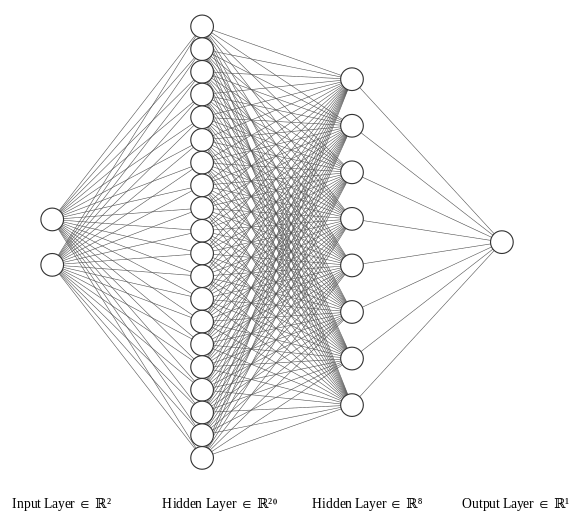
\includegraphics[width=0.9\textwidth]{figures/ann_2.png}
\caption{Graphical representation of the ANN used to approximate the Black and Scholes option price function.}
\label{fig:ann_2}
\end{figure}

\begin{ipython}
X_scaled = scale_X.fit_transform(df[['vol', 'rate']])
Y_scaled = scale_Y.fit_transform(df[['price']])
	
X_train, X_test, Y_train, Y_test = train_test_split(X_scaled, 
                                                    Y_scaled, test_size=0.2)

model = Sequential()
model.add(Dense(20, input_dim=2, activation='relu'))
model.add(Dense(8, activation='relu'))
model.add(Dense(1, activation='relu'))

model.compile(loss='mse', optimizer='adam')
model.fit(X_train, Y_train, epochs=1500, verbose=1)
\end{ipython}
\begin{ioutput}
Epoch 1/1500
250/250 [==============================] - 1s 1ms/step - loss: 0.0583
Epoch 2/1500
250/250 [==============================] - 0s 1ms/step - loss: 0.0042
...
Epoch 1499/1500
250/250 [==============================] - 0s 2ms/step - loss: 4.5252e-07
Epoch 1500/1500
250/250 [==============================] - 0s 2ms/step - loss: 4.8000e-07
<keras.callbacks.History at 0x7efd8c4dd7d0>
\end{ioutput}

\begin{ipython}
eval1 = model.evaluate(X_train, Y_train)
print('Training: {}'.format(eval1))

eval2 = model.evaluate(X_test, Y_test)
print('Test: {}'.format(eval2))
\end{ipython}
\begin{ioutput}
250/250 [==============================] - 0s 1ms/step - loss: 5.9946e-07
Training: 5.994579055368376e-07
63/63 [==============================] - 0s 2ms/step - loss: 6.0690e-07
Test: 6.06896833232895e-07
INFO:tensorflow:Assets written to: bs_model/assets
['bs_model_y_scaler.save']
\end{ioutput}

As you can see the training and testing samples give roughly the same loss value so we can be reasonably sure that there hasn't been \emph{overfitting}.
After we can evaluate graphically how good is the training by plotting the difference between predicted and target output as a function of the input parameters, see Figure~\ref{fig:vol_rate}. 
The gibbous structure of the relative error distribution, shown by Fig.~\ref{subfig:rel_err}, most likely can be flatten out with longer (hence more precise) training. The large peak in the low rate/volatility region is instead due to the decreasing price of the call: the absolute error (see Fig.~\ref{subfig:abs_err}) is quite flat in that region and the decreasing price (it actually tends to zero there, see Fig.~\ref{subfig:shape}) boosts the relative error.

\begin{figure}[!htp]
\centering
\subfloat[Black-Scholes price (at-the-money call). \label{subfig:shape}]{%
	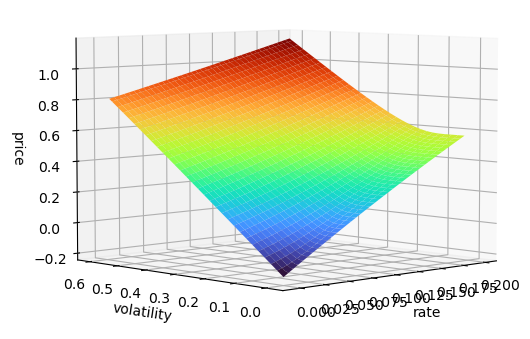
\includegraphics[width=0.7\textwidth]{figures/bs_shape}
	}\\[30pt]
\subfloat[Relative error between predicted and actual price. \label{subfig:rel_err}]{%
	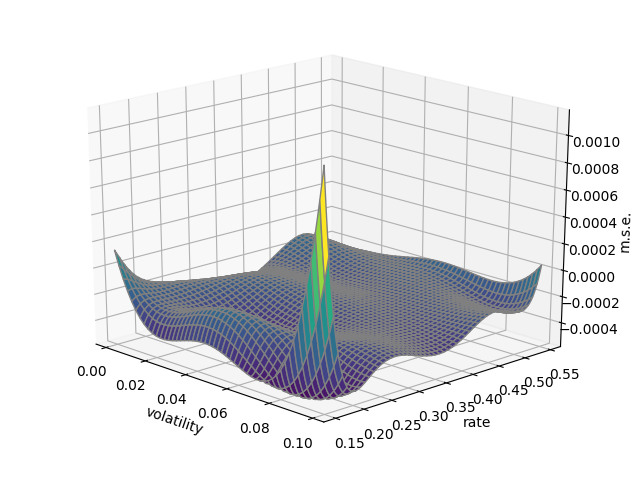
\includegraphics[width=0.5\textwidth]{figures/vol_rate}
	}
\subfloat[Absolute errror between predicted and actual price. \label{subfig:abs_err}]{%
    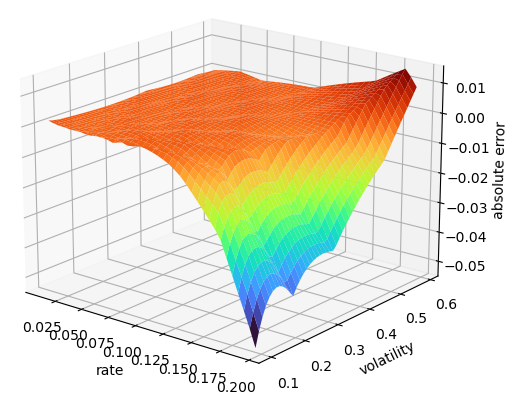
\includegraphics[width=0.5\textwidth]{figures/vol_rate_abs_err}
	}
\caption{Neural network performance.}
\label{fig:vol_rate}
\end{figure}

When you are satisfied by the results don't forget to save the model and the scalers for later usage.

\begin{ipython}
import joblib

eval1 = model.evaluate(X_train, Y_train)
print('Training: {}'.format(eval1))

eval2 = model.evaluate(X_test, Y_test)
print('Test: {}'.format(eval2))

job_name = 'bs_model'
model.save(job_name)
joblib.dump(scale_X, job_name + "_x_scaler.save")
joblib.dump(scale_Y, job_name + "_y_scaler.save")
\end{ipython}

\subsection{Option Price Estimate}
Say we want to know the price of an at-the-money, 1 year call when the risk-free rate is 0.015 and the underlying volatility 0.234. Before feeding the inputs into the neural network we need to transform them using the same scalers used before the training, otherwise the range of the inputs is not interpreted correctly by the model. Similarly the result of the prediction has to undergo the inverse transformation applied for the training to the output in order to have the actual option price.

\begin{ipython}
import numpy as np
from finmarkets import call_m
from keras.models import load_model

model = load_model(job_name)
scale_X = joblib.load(job_name + "_x_scaler.save")
scale_Y = joblib.load(job_name + "_y_scaler.save")

vr = np.array([[0.234, 0.015]])
prediction = model.predict(scale_X.transform(vr))
prediction = scale_Y.inverse_transform(prediction)[0][0]
call_price = call_m(1, vr[0][0], vr[0][1], 1)

print ('{} => {:.4f} (expected {:.4f})'.format(vr.tolist(), prediction, call_price))
\end{ipython}
\begin{ioutput}
[[0.234, 0.015]] => 0.0999 (expected 0.1001)
\end{ioutput}

It is very important to remark that a \textbf{NN cannot extrapolate}. Indeed if you try to predict the price of an option from rate and volatility outside the training \emph{phase space} (i.e. with values that aren't in the intervals used in the training), say $r = 0.22$ and $\sigma = 0.01$

\begin{ipython}
vr = np.array([[0.22, 0.01]])
prediction = model.predict(scale_X.transform(vr))
prediction = scale_Y.inverse_transform(prediction)[0][0]
call_price = call_m(1, vr[0][0], vr[0][1], 1)

print ('{} => {:.4f} (expected {:.4f})'.format(vr.tolist(), prediction, call_price))
\end{ipython}
\begin{ioutput}
[[0.22, 0.01]] => 0.1583 (expected 0.1975)
\end{ioutput}

So in this case the NN prediction is completely wrong.

\section{Model Calibration}\label{model-calibration}

To use a certain model to solve real-world problems it is necessary to \emph{calibrate} it. This means that model parameters are derived directly from current market values. 

\begin{attention}
\subsubsection{Historical vs. Implied Volatility}
\label{historical-vs.-implied-volatility}
	
\emph{Historical volatility} is the realized volatility of an asset over a previous time period. It is determined by measuring the standard deviation of its price during that time period.
	
\emph{Implied volatility} is the expected future volatility of an asset that is implied by the current price of market products involving it.
In contrast to historical volatility, which looks at prices in the past, implied volatility looks toward the future and is often interpreted as the market's expectation for the future volatility of an asset.
	
Volatility shifts as market goes through different regimes, thus, historical volatility may not be an accurate estimate of future. Implied volatility instead takes into account all information used by market participants to determine the prices and can give indications on the future behaviour.
\end{attention}

Assume we need to estimate the \emph{implied volatility} of a security and that we don't know any analytic expression for it. We could train a neural network to approximate this unknown function, which is the inversion of the Black-Scholes formula returning the volatility given the option price

\begin{equation} 
\sigma = F^{-1}_\textrm{BS}(P_\textrm{call}, m, r, \mathrm{ttm})
\end{equation}

In this case calibration means to determine one of the Black-Scholes formula parameter (the volatility) from the market prices of the options and their characteristics.

The training sample created before can be used this time by swapping its columns to have in input rate and option price and as the target output the volatility. Indeed we have never made any assumption on the functional form of the expression to approximate but just relied on the capability of NN to learn from the dataset, so this should be enough.
This is very convenient to estimate quantities which are otherwise complicated to compute (i.e. there is no analytic formula to determine them).
 
\begin{ipython}
import pandas as pd

df = pd.read_csv("bs_training_sample.csv")
scale_X = MinMaxScaler()
scale_Y = MinMaxScaler()
X_scaled = scale_X.fit_transform(df[['rate', 'price']])
Y_scaled = scale_Y.fit_transform(df[['vol']])

X_train, X_test, Y_train, Y_test = train_test_split(X_scaled, 
                                                    Y_scaled, test_size=0.2)

model = Sequential()
model.add(Dense(20, input_dim=2, activation='relu'))
model.add(Dense(8, activation='relu'))
model.add(Dense(1, activation='relu'))

model.compile(loss='mse', optimizer='adam')
model.fit(X_train, Y_train, epochs=1500, verbose=1)

eval1 = model.evaluate(X_train, Y_train)
print('Training: {}'.format(eval1))

eval2 = model.evaluate(X_test, Y_test)
print('Test: {}'.format(eval2))
\end{ipython}
\begin{ioutput}
Epoch 1/2000
8000/8000 [==============================] - 0s 14us/step - loss: 0.1339
Epoch 2/2000
8000/8000 [==============================] - 0s 4us/step - loss: 0.1052
...
Epoch 1499/1500
250/250 [==============================] - 0s 2ms/step - loss: 3.8106e-07
Epoch 1500/1500
250/250 [==============================] - 0s 2ms/step - loss: 3.1316e-07
<keras.callbacks.History at 0x7efd8c5dea10>

250/250 [==============================] - 0s 1ms/step - loss: 2.8773e-07
Training: 2.8773044391527947e-07
63/63 [==============================] - 0s 2ms/step - loss: 2.9526e-07
Test: 2.9526071898544615e-07
INFO:tensorflow:Assets written to: calibration_model/assets
['calibration_model_y_scaler.save']
\end{ioutput}

We can now estimate the implied volatility assuming a risk-free rate of 2\% and the current option price equal to 0.15 

\begin{ipython}
rp = np.array([[0.02, 0.15]])
prediction = model.predict(scale_X.transform(rp))
volatility = scale_Y.inverse_transform(prediction)[0][0]

print ('{} => {:.4f} (expected call price {:.4f})'.format(rp.tolist(), 
                                                          volatility, 
                                                          call_m(1, volatility, 
                                                                 0.02, 1)))
\end{ipython}
\begin{ioutput}
[[0.02, 0.15]] => 0.3557 (expected call price 0.1499)
\end{ioutput}
\noindent
The expected call price derived using the estimated implied volatility (0.1499) is in excellent agreement we the market price (0.15).

\section{Bankruptcy Prediction}
A company faces bankruptcy when it is unable to pay off its debts. The Taiwan Economic Journal has listed the details of company bankruptcy for the years between 1999 to 2009 based on the business regulations of the Taiwan Stock Exchange which is a local financial institution. The dataset includes 94 numerical attributes that help understand the possibility of bankruptcy.

This NN application aims at analyzing the possibility of whether an organization would face bankruptcy. This is a typical classification problem and the model output will be a number representing the probability of default of a given company.
Beside that a couple more concepts are analyzed in this example:
\begin{itemize}
\item \emph{imbalanced datasets}: is a situation when there is an unequal distribution of classes in a dataset. It can be solved by either up-sampling (i.e. introducing minority class samples) or down-sampling (i.e. reducing majority class to match the size of minority class);
\item finding the best attributes to work with through feature selection (i.e. it will be shown how programatically pick the best features).
\end{itemize}

The input dataset can be downloaded from \href{https://raw.githubusercontent.com/matteosan1/finance_course/develop/libro/input_files/bankruptcy_data.csv}{bankruptcy\_data.csv}
\begin{ipython}
import pandas as pd
	
data = pd.read_csv("bankruptcy_data.csv")	
print (data.head())
\end{ipython}
\begin{ioutput}
Net Worth Turnover Rate (times)  Revenue per person  \
0                          0.03                0.03   
1                          0.03                0.01   
2                          0.01                0.03   
3                          0.03                0.02   
4                          0.04                0.06   
	
Operating profit per person  Allocation rate per person  \
0                      0.39                        0.04   
1                      0.39                        0.01   
2                      0.38                        0.14   
3                      0.38                        0.02   
4                      0.39                        0.02   

Working Capital to Total Assets  Quick Assets/Total Assets  \
...                        
\end{ioutput}

Given the very large number of available features it could be useful to remove those which present high correlation with other features in the set (i.e. are redundant) and therefore cannot bring much improvement to the NN performance.

Two techniques can be used: either perform a principal component analysis on the dataset and just keep the highest ranked features of the most significant component~\ref{sec:PCA} or compute the correlation matrix of the features, set a threshold, and remove all the attributes above this value.

Here the latter method is used, choosing a correlation threshold of $|\rho|\geq 0.95$.

\begin{ipython}
corr_mat = data.corr()
corr_mat = corr_mat.iloc[1:, 1:]
	
drop_list = {}
for i in range(len(corr_mat.columns)):
    for j in range(i):
        if abs(corr_mat.iloc[i, j]) >= 0.95:
            if corr_mat.columns[j] not in drop_list:
                drop_list.setdefault(corr_mat.columns[j], []) \
                    .append(corr_mat.columns[i])

for d in drop_list.keys():
    print (d)
\end{ipython}
\begin{ioutput}
ROA(C) before interest and depreciation before interest
ROA(A) before interest and % after tax
Operating Gross Margin
Pre-tax net Interest Rate
After-tax net Interest Rate
Net Value Per Share (B)
Net Value Per Share (A)
Persistent EPS in the Last Four Seasons
After-tax Net Profit Growth Rate
Debt ratio %
Operating Profit Per Share (Yuan)
Per Share Net profit before tax (Yuan)
Current Liabilities/Liability
Current Liabilities/Equity
Realized Sales Gross Margin
Borrowing dependency
Current Liability to Equity
\end{ioutput}
\noindent 
By analysing \texttt{drop\_list} it could also be checked where the maximum correlation happens.

Those 17 attributes are highly correlated with others in the dataset, therefore they do not bring additional discrimination power to the network and can be safely discarded. To check the effect of removing columns from a dataset NN performance should be compared with and without the selected attributes. Here for simplicity this step will be skipped assuming there is an improvement.

\begin{ipython}
data = data.drop(drop_list, axis=1)
y = data['Bankrupt?']
X = data.drop(['Bankrupt?'], axis=1)
\end{ipython}

\subsection{Unbalanced Datasets}

\begin{ipython}
print (data['Bankrupt?'].value_counts())
\end{ipython}
\begin{ioutput}
0    6599
1     220
Name: Bankrupt?, dtype: int64
\end{ioutput}

From the above check it is apparent that the dataset is highly imbalanced (i.e. large majority of companies didn't default). The main problem with imbalanced classification is that there are too few examples of the minority class for a model to effectively learn the decision boundary. 

To patch this issue it has been decided to apply an oversampling method called Synthetic Minority Oversampling Technique (SMOT)~\cite{bib:smot}. 

\begin{attention}
Oversampling could be in principle achieved by simply duplicating samples from the minority class in the training dataset prior to fitting a model. This would balance the class distribution but wouldn't provide any additional information to the model since it is merely a duplication of the existing information.
	
An improvement with respect to this trivial strategy is to synthesize new samples from the minority class, a type of data augmentation that can be very effective.

SMOT algorithm works as follows: a random sample $x$ from the minority class is chosen. Then $k$ of the nearest neighbors of $x$ are found (typically $k=5$) and one of them is randomly selected. Finally a synthetic sample is created at a random point in the feature space between the two samples.
%Figure~\ref{fig:smote} shows an example of the algorithm.

%begin{figure}[htb]
\begin{center}
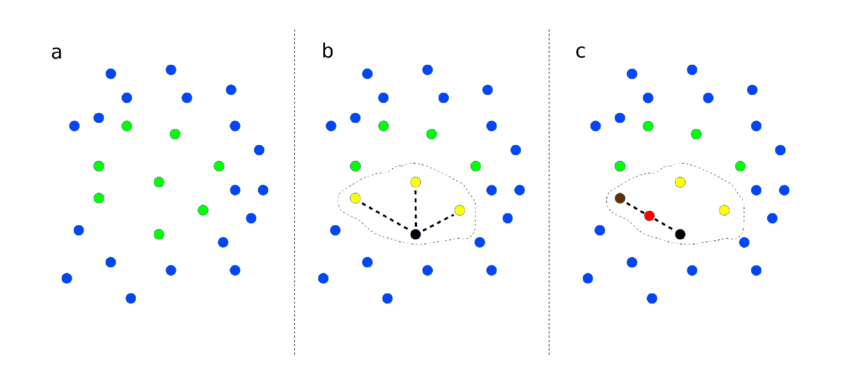
\includegraphics[width=0.7\textwidth]{figures/smote}
\captionof{figure}{Graphical representation of the SMOT algorithm.}
%\label{fig:smote}
\end{center}

This procedure can be used to create as many synthetic samples for the minority class as required. The approach is effective because new synthetic samples are plausible, that is, are relatively close in feature space to existing samples from the minority class.

A general downside of the approach is that synthetic samples are created without considering the majority class, possibly resulting in ambiguous samples if there is a strong overlap for the classes.
\end{attention}

In \texttt{python} SMOT is implemented in \texttt{imblearn.over\_sampling} module.

\begin{ipython}
from imblearn.over_sampling import SMOTE
	
oversample = SMOTE()
X_sm, y_sm = oversample.fit_resample(X, y)
print (y_sm.value_counts())
\end{ipython}
\begin{ioutput}
1    6599
0    6599
Name: Bankrupt?, dtype: int64
\end{ioutput}

The last step to prepare the dataset for the analysis is its normalization which is necessary since each feature column ranges very differently.

\begin{ipython}
from sklearn.preprocessing import StandardScaler
from sklearn.model_selection import train_test_split

scaler = StandardScaler()
X_sm = scaler.fit_transform(X_sm)

X_train, X_test, y_train, y_test = train_test_split(X_sm, y_sm, test_size=0.2)
\end{ipython}

Now we can define the neural network architecture and go on with the training. An early stopping \emph{callback} has been implemented in order to stop the training in case no significant improvement is observed in the last 50 epochs in terms of loss reduction.

In computer programming, a callback is any executable code that is passed as an argument to other code; that other code is expected to execute at a given time.

\begin{ipython}
from tensorflow.keras.layers import Dropout
from tensorflow.keras.callbacks import EarlyStopping
	
model = Sequential()
	
model.add(Dense(77, activation='relu'))
model.add(Dropout(0.3))
model.add(Dense(77, activation='relu'))
model.add(Dropout(0.3))
model.add(Dense(1, activation='sigmoid'))
	
model.compile(loss='binary_crossentropy', optimizer='adam')
	
early_stop = EarlyStopping(monitor='val_loss', 
                           mode='min', 
                           verbose=1, 
                           patience=50)
	
model.fit(X_train, y_train,
          epochs=600,
          validation_data=(X_test, y_test), 
          verbose=1, callbacks=[early_stop])
          
loss = model.history.history['loss']
val_loss = model.history.history['val_loss']
\end{ipython}
\begin{ioutput}
Epoch 1/600
330/330 [==============================] - 2s 4ms/step - loss: 0.3348 
- val_loss: 0.2354
Epoch 2/600
330/330 [==============================] - 1s 3ms/step - loss: 0.2318 
- val_loss: 0.2007
...
Epoch 176/600
330/330 [==============================] - 1s 3ms/step - loss: 0.0142 
- val_loss: 0.0670
Epoch 177/600
330/330 [==============================] - 1s 2ms/step - loss: 0.0069 
- val_loss: 0.0640
Epoch 00177: early stopping
<keras.callbacks.History at 0x7f07928fd150>
\end{ioutput}

\begin{attention}
\subsubsection{Dropout}
Large neural nets trained on relatively small datasets tend to overfit.

In this case the model is learning the statistical noise in the training data, so it results in poor performance when the model is evaluated on new data (e.g. the test dataset).

One approach to reduce overfitting is to fit all possible different neural networks on the same dataset and to average the predictions from each model. This is not feasible in practice, and can be approximated using a small collection of different models, called an ensemble. A problem even with the ensemble approximation is that it requires multiple models to be fit and stored, which can be a challenge if the models are large, requiring days or weeks to train and tune.

\emph{Dropout} is a regularization method that approximates training a large number of neural networks with different architectures in parallel.

During training, some number of layer outputs are randomly ignored or \emph{dropped out}. This has the effect of making the layer look like and treated like a layer with a different number of nodes and connectivity to the prior layer. In effect, each update to a layer during training is performed with a different "view" of the configured layer.

Even if it may seems counter intuitive (better training when switching off nodes) indeed dropout breaks up situations where network layers co-adapt to correct mistakes from prior layers, in turn making the model more robust.
\end{attention}

Figure~\ref{fig:bankruptcy_loss} reports the loss function values, in training and testing samples, versus the epoch number. From the plot it is clear how there is no significant improvement after epoch 30 in the testing sample, that's why the training is stopped early.

\begin{figure}[htbp]
\centering
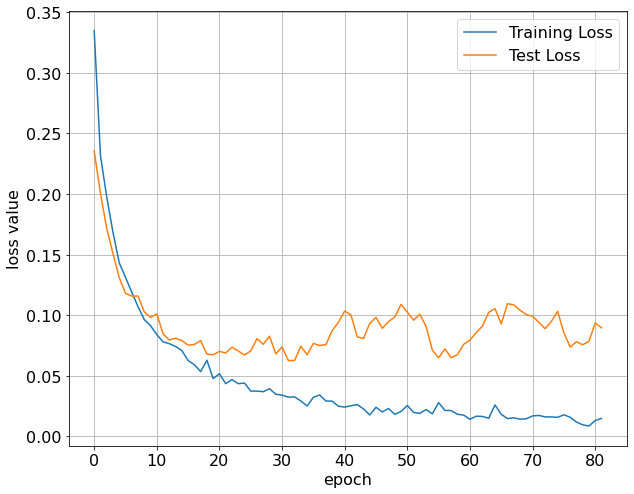
\includegraphics[width=0.7\linewidth]{figures/bankruptcy_loss}
\caption{Loss value as a function of the number of epochs in training and testing sample.}
\label{fig:bankruptcy_loss}
\end{figure}

Performance-wise a classification NN can be evaluated using the so called \emph{confusion matrix} plot shown in Figure~\ref{fig:confusion_matrix}. This is a matrix that compares the number of actual and predicted events in each category, reporting true and false predictions. In case of only two classes it becomes:

\begin{equation*}
\begin{bmatrix}
	TP & FP \\
	FN & TN  
\end{bmatrix}
\end{equation*}
\noindent
where $TP$ is the number of true "positive", $FN$ that of false "negative" and so on.

\begin{ipython}
from sklearn.metrics import confusion_matrix, ConfusionMatrixDisplay
	
predictions = (model.predict(X_test) > 0.5).astype("int32")
	
cm = confusion_matrix(y_test, predictions)
cmd_obj = ConfusionMatrixDisplay(cm, display_labels=['No Bankruptcy', 'Bankruptcy'])
cmd_obj.plot()
cmd_obj.ax_.set(title='', xlabel='Predicted', ylabel='Actual')
plt.show()
\end{ipython}
\noindent
From this matrix a number of information can be determined~\cite{bib:sensitivity}:

\makegapedcells\begin{table}[htbp]
\centering
\begin{tabular}{|l|c|c|}
\hline
Mis-classification (error rate) & $\cfrac{FP+FN}{n}$ & 0.8\% \\
\hline
Sensitivity (true positive) & $\cfrac{TP}{FN+TP}$ & 99.9 \% \\
\hline
False positive & $\cfrac{FP}{TN+FP}$ & 1.5\% \\
\hline
Specificity (true negative) & $\cfrac{TN}{TN+FP}$ &  98.5\% \\
\hline
False negative & $\cfrac{FN}{TP+FN}$ & 0.08\% \\
\hline
Precision & $\cfrac{TP}{FP+TP}$ & 98.4\% \\ 
\hline
Accuracy & $\cfrac{TN+TP}{n}$ & 99.2\% \\
\hline
\end{tabular}
\end{table}

\begin{figure}[htbp]
\centering
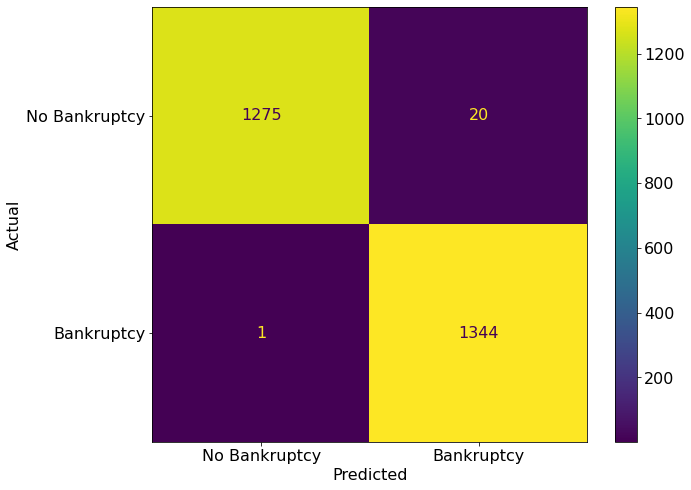
\includegraphics[width=0.7\linewidth]{figures/confusion_matrix}
\caption{Confusion matrix for the evaluation of the ANN to predict bankruptcy events.}
\label{fig:confusion_matrix}
\end{figure}

Since the goal was to train a neural network to predict company bankruptcy the most interesting parameters are the \emph{specificity} which is pretty high (98.5\%) and the \emph{false negative rate} which contrary is very small ($\lt 0.1\%$).

%\section{Model Calibration cont.}
%\label{model-calibration-cont.}

%When a model has just three known parameters a convolutional neural network can be used to calibrate it.
%
%Consider again the Black-Scholes formula and imagine you need to calibrate: rate $r$ and volatility $\sigma$ at the same time.
%
%A black-white image can be interpreted as a map where each pixel coordinates is a pair ($\mathrm{ttm}, M$) and the pixel color, an integer between 0 (black) and 255 (white), represents \(P_\textrm{call}\). Each picture will be classified by a pair of $r, \sigma$.
%
%The creation of the training sample is a little more complicated now. For convenience we will use also a new format to save data image, \texttt{numpy}. This will be done through the corresponding module simply using the functions \texttt{save} and \texttt{load} to store and retrieve data. The module \texttt{PIL} (\texttt{pillow}) is instead used to visualize the images.
%
%First make the targets.
%
%\begin{ipython}
%import numpy as np
%from finmarkets import call_m
%
%labels = []
%rates = np.arange(0.01, 0.11, 0.001)
%vols = np.arange(0.1, 0.6, 0.005)
%for i in range(len(vols)):
%    for j in range(len(rates)):
%        labels.append((vols[i], rates[j]))
%\end{ipython}
%\noindent
%Then we can create the images.
%
%\begin{ipython}
%k = np.arange(0.8, 1.2, (1.2-0.8)/20)
%ttm = np.arange(1, 5, 4/20)
%
%# for each r, sigma pair
%# generate a matrix of prices
%maximum = 0
%minimum = np.inf
%prices = []
%for v in vols:
%    for r in rates:
%        price = np.zeros(shape=(20, 20))
%        for ik, kv in enumerate(k):
%            for it, t in enumerate(ttm):
%                price[ik, it] = call_m(kv, r, v, t)
%                prices.append(price)
%                # max and min are saved to
%                # normalize our matrices
%                new_max = np.max(price)
%                new_min = np.min(price)
%                if new_max > maximum:
%                    maximum = new_max
%                if new_min < minimum:
%                    minimum = new_min
%for ip, p in enumerate(prices):
%    prices[ip] = np.interp(p, (minimum, maximum), (0, 1))
%np.save("2d", prices)
%\end{ipython}
%\noindent
%An example of the 20x20 images that have been created is shown in Fig.~\ref{fig:test_images_calib}.
%
%\begin{figure}[htb]
%\centering
%
\includegraphics[width=0.45\textwidth]{figures/2d_training_images}
%\caption{Example of images used to encode calibration information.}
%\label{fig:test_images_calib}
%\end{figure}
%\noindent
%Then the training is similar to what has been done for the handwritten digits.
%
%\begin{ipython}
%import numpy as np
%from finnn import FinNN
%
%labels = np.load("2d_labels.npy")
%images = np.load("2d.npy")
%
%trainer = FinNN("CNN2D")
%trainer.setData(images, labels, test_size=0.2)
%trainer.addConv2DLayer(filters=8, filter_size=10,
%                       input_shape=(20, 20, 1), activation='relu')
%trainer.addFlatten()
%trainer.addHiddenLayer(neurons=10, activation='relu')
%trainer.addOutputLayer(outputs=2, activation='relu')
%
%trainer.compileModel(loss='mse', opt='adam')
%trainer.fit(epochs=500, verbose=1)
%trainer.saveModel("2d")
%trainer.evaluate()
%\end{ipython}
%\begin{ioutput}
%Epoch 1/500
%8000/8000 [==============================] - 1s 156us/step - loss: 0.0018
%Epoch 2/500
%8000/8000 [==============================] - 1s 142us/step - loss: 6.2310e-04
%...
%Epoch 499/500
%8000/8000 [==============================] - 2s 194us/step - loss: 1.4921e-06
%Epoch 500/500
%8000/8000 [==============================] - 2s 193us/step - loss: 1.4413e-06
%
%8000/8000 [==============================] - 1s 65us/step
%Training: 1.1013161047230825e-05
%2000/2000 [==============================] - 0s 70us/step
%Test: 1.116331470257137e-05
%\end{ioutput}
%
%At this point the test of the trained CNN consists of presenting the prices of call referring to the same underlying in the pictorial form shown before and in response it will give the risk-free rate and the volatility.
%
%\begin{ipython}
%for i in range(5):
%    print (trainer.predict(trainer.x_test[i:i+1]))
%\end{ipython}
%\begin{ioutput}
%[[0.3825101  0.09229672]]
%[[0.4056808  0.02232919]]
%[[0.47402808 0.05630913]]
%[[0.2851617  0.05214534]]
%[[0.17245176 0.08815573]]
%\end{ioutput}

\section{Technical Analysis}
\label{technical-analysis}

In finance \emph{technical analysis} is a discipline for forecasting the direction of prices through the study of past market data, primarily price and volume. The analysts look for particular patterns in the price series that are \emph{believed} to develop in a predictable way. Fig.~\ref{fig:tech_ana} shows two of such patterns.

\begin{figure}[htb]
\centering
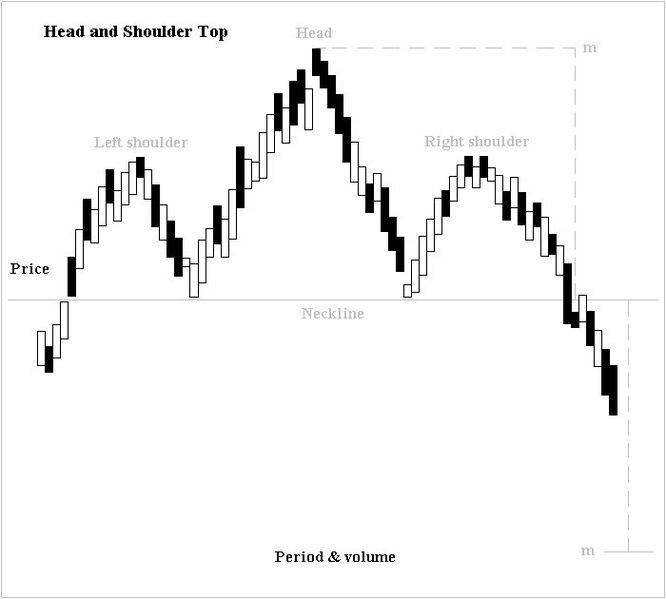
\includegraphics[width=0.4\linewidth]{figures/H_and_s_top_new.jpg}\qquad
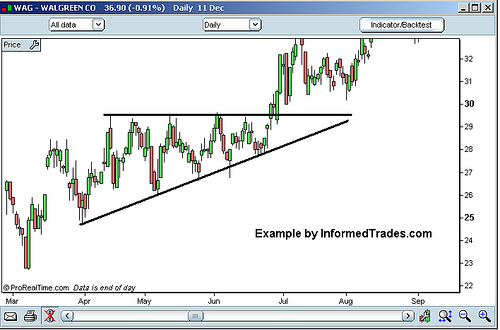
\includegraphics[width=0.4\linewidth]{figures/Triangle-ascending.jpg}
\caption{Examples of patterns in real time series, head and shoulder (left), triangle (right).}
\label{fig:tech_ana}
\end{figure}

We will develop a (1D) CNN capable of classifying features in time series to be used in technical analysis (which is much faster than having somebody looking at thousands of time series by eye).

The training sample is made of 21600 time series (1/3 with head and shoulder patter, 1/3 with triangle pattern and 1/3 with no pattern), for an example see Fig~\ref{fig:patterns}. Notice that to make the training easier plot features are quite exaggerated.

Images and corresponding labels are stored in \href{https://drive.google.com/file/d/1lx8l6MQCfBtzjdVK-qvwDxzP3Eh5eONR/view?usp=sharing}{training\_techana\_labels.npy} and
\href{https://drive.google.com/file/d/1Vt4XJfDu6FiPGAKuEu-2m4MMCgBjY_eN/view?usp=sharing}{training\_techana\_images.npy}

\begin{figure}[htbp]
\centering
\subfloat[No pattern.\label{}]{%
	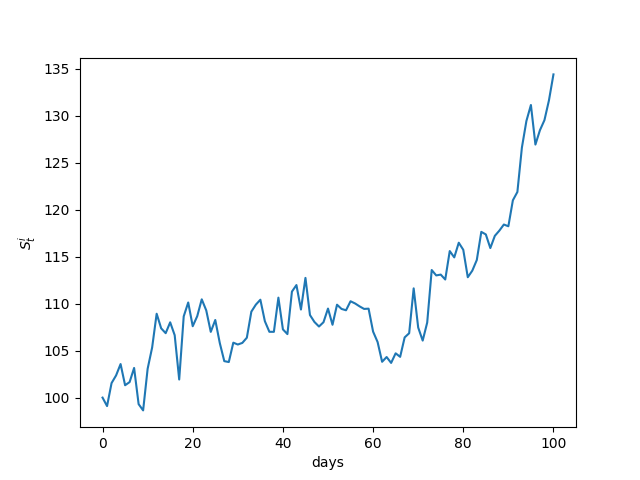
\includegraphics[width=0.5\textwidth]{figures/no_pattern}
}
\subfloat[Head and shoulder pattern.\label{}]{%
	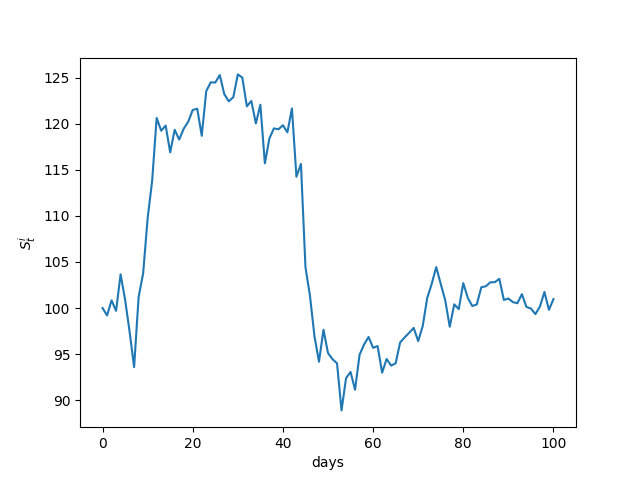
\includegraphics[width=0.5\textwidth]{figures/head_and_shoulder}
}\\
\subfloat[Triangle pattern.\label{}]{%
	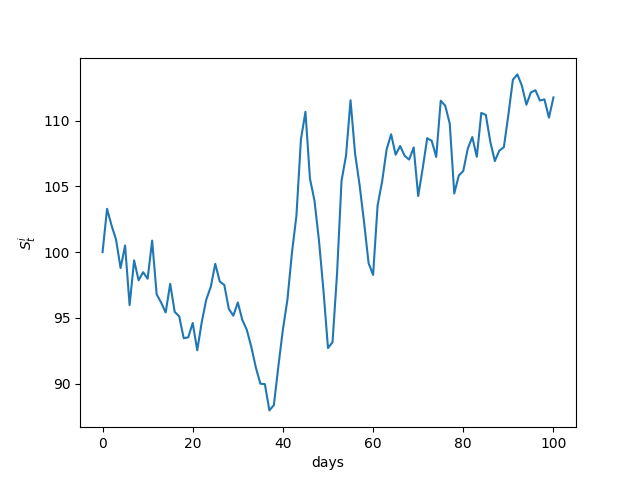
\includegraphics[width=0.5\textwidth]{figures/triangle}
}
\caption{Examples of time series used in the training of the CNN for technical analysis.}
\label{fig:patterns}
\end{figure}

\begin{ipython}
import numpy as np
from keras.models import Sequential
from keras.layers import Dense, Conv1D, Dropout, MaxPooling1D, GlobalAveragePooling1D
from tensorflow.keras.utils import to_categorical

train_labels = np.load("training_techana_labels.npy")
train_images = np.load("training_techana_images.npy")

model = Sequential()
model.add(Conv1D(filters=80, kernel_size=20, 
activation='relu', input_shape=(101, 1)))
model.add(Conv1D(filters=80, kernel_size=15, activation='relu')) 
model.add(MaxPooling1D(3))
model.add(Conv1D(filters=100, kernel_size=10, activation='relu'))
model.add(Conv1D(filters=100, kernel_size=5, activation='relu'))
model.add(GlobalAveragePooling1D())
model.add(Dropout(0.5))
model.add(Dense(3, activation='softmax'))

model.compile(loss='categorical_crossentropy', optimizer='adam')
self.model.fit(train_images, to_categorical(train_labels), epochs=80)
\end{ipython}
\begin{ioutput}
Epoch 1/80
- 23s 1ms/step - loss: 0.6773
Epoch 2/80
- 23s 1ms/step - loss: 0.5421
...
Epoch 79/80
- 26s 39ms/step - loss: 0.0699
Epoch 80/80
- 27s 40ms/step - loss: 0.0584
\end{ioutput}

CNN performance are checked by simulating incoming data in "real-time" as in a real case scenario . The goal is to recognize any pattern as soon as possible. 

The simulation is carried on presenting to the CNN sliding time windows of the time series
\begin{itemize}
	\item at $t_1$ the input is represented by the points between $[0, 80]$;
	\item at $t_2$ by the points between $[1, 81]$;
	\item at $t_3$ between $[2, 82]$ and so on.
\end{itemize}

Figure~\ref{fig:frame_simulation} shows the "temporal frames" that have been presented to the CNN and which are stored in \href{https://drive.google.com/file/d/1924W_OiOYmFQ53sCirG-k3FyekgUl9Wr/view?usp=sharing}{testing\_techana\_frames.npy}.

\begin{figure}
\centering
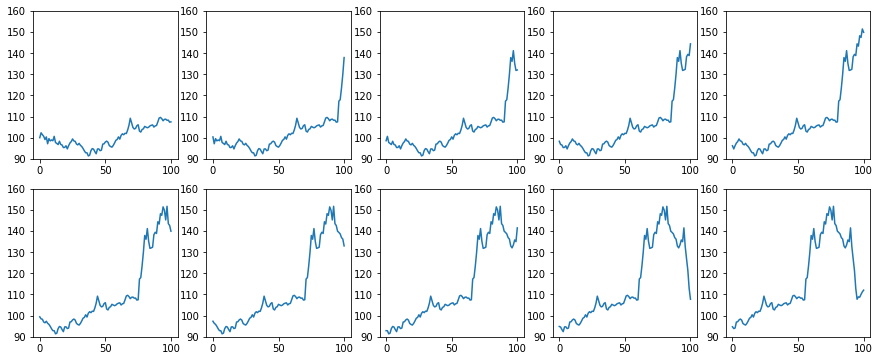
\includegraphics[width=\textwidth]{figures/tech_ana_frames}
\caption{Ten frames simulating price data incoming in real time. The CNN was tested to check if and when it would have been able to detect any pattern in it.}
\label{fig:frame_simulation}
\end{figure}

\begin{ipython}
test_images = np.load("testing_techana_frames.npy")
predictions = model.predict(test_images)

for i in range(len(predictions)):
    print (np.argmax(predictions[i]), ["{:.3f}".format(p) for p in predictions[i]])
\end{ipython}
\begin{ioutput}
0 ['0.942', '0.000', '0.058']
0 ['0.970', '0.000', '0.030']
0 ['1.000', '0.000', '0.000']
0 ['0.999', '0.001', '0.000']
0 ['0.784', '0.216', '0.000']
1 ['0.000', '1.000', '0.000']
1 ['0.000', '1.000', '0.000']
1 ['0.000', '1.000', '0.000']
1 ['0.000', '1.000', '0.000']
1 ['0.000', '1.000', '0.000']
\end{ioutput}
\noindent
The output represents the likelihood that the time series belongs to any category at each time. Up to $t=4$ the CNN is about 95\% sure that there is no pattern (max probability at category 0). 
At $t=5$ the CNN starts recognizing a pattern assigning about 20\% probability to the "head and shoulders" class. For $t\geq 6$ the neural network is about 100\% sure of the pattern.

\section{Unsupervised Learning}
    
Unsupervised learning is a type of machine learning in which the algorithm is not provided with any pre-assigned labels or scores for the training data. As a result, unsupervised learning algorithms must self-discover any naturally occurring pattern in that training data set. 
    
Quite common examples of unsupervised learning are \emph{clustering}, where the algorithm automatically groups the training examples into categories with similar features, and \emph{principal component analysis}~\ref{sec:pca}, where the algorithm finds ways to compress the training data set by identifying which features are most useful for discriminating between different training examples, and discarding the rest. 
    
\subsection{k-Means Algorithm}
    
k-means clustering~\cite{bib:k-means} is a method of vector quantization that aims to partition (split) $n$ observations into $k$ clusters in which each observation belongs to the cluster with the nearest "mean" (cluster centers or cluster centroid). 
    
Given a set of observations $(x_1, x_2, \ldots, x_n)$, where each one is a $d$-dimensional vector, the algorithm divides the $n$ observations into $k \leq n$ sets $S = \{S_1, S_2, \ldots, S_k\}$ such to minimize the within-cluster sum of squares (i.e. variance). Formally, the objective is to find:
    
\begin{equation}
\underset {\mathbf {S}}{\operatorname {arg\,min} } \sum _{i=1}^{k}\sum _{\mathbf {x} \in S_{i}}\left\|\mathbf {x} -{\boldsymbol {\mu }}_{i}\right\|^{2}
\end{equation}
where $μ_i$ is the mean of points in $S_i$. 
    
\subsubsection{Example}
This example consists of clustering a dataset that contains information of all the stocks that compose the SP500 Index. 
    
The input dataset, fetched from Yahoo Finance and stored in \href{https://github.com/matteosan1/finance_course/raw/develop/libro/input_files/k\_mean.csv}{k\_mean.csv}, is made of the daily closing prices of each share within the interval 2018-09-20, 2021-09-20.
    
The goal of this study is to find similarities among companies in terms of return and volatility. To do this, the k-means clustering algorithm will assign a label, representing the clusters, to each company.
 
The first step is loading the inputs (from \href{https://github.com/matteosan1/finance_course/blob/develop/libro/input_files/k_mean.csv?raw=true}{k\_mean.csv}) and produce a new \texttt{DataFrame} with annualized returns and volatilities for each stock. 
 
\begin{ipython}
import pandas as pd
 
df = pd.read_csv("k_mean.csv", index_col='Date')
 
returns = df.pct_change().mean()*252
std = df.pct_change().std()*np.sqrt(252)
 
ret_var = pd.concat([returns, std], axis=1)
ret_var = ret_var.dropna()
ret_var.columns = ["Returns","Standard Deviation"]
print (ret_var.head())
\end{ipython}
\begin{ioutput}
       Returns  Standard Deviation
MMM  -0.188903            0.261649
ABT   0.235801            0.232519
ABBV -0.159596            0.304667
ABMD -0.543486            0.526830
ACN   0.152511            0.212579
\end{ioutput}

\subsection{Elbow Curve}
 
In order to determine the optimal number of clusters $k$ to look for in our dataset, we will fit different models of the k-means algorithm while varying the $k$ parameter in the range $[2, 14]$. For each model we calculate the Sum Squared Error (SSE) by using the \texttt{.inertia\_\_} method of model. "Inertia" tells how far away the points within a cluster are, the smaller the inertia the better.
 
Each pair of values ($k$, SSE) will help to construct the \emph{Elbow Curve}~\cite{bib:elbow_curve} which can be used to determine the optimal value for $k$. 
 
Using the "elbow" or "knee" of a curve as a cutoff point is a common heuristic in mathematical optimization to choose a point where diminishing returns are no longer worth the additional cost. In clustering, this means one should choose a number of clusters so that adding another cluster doesn't give much better modeling of the data.
 
The intuition is that increasing the number of clusters will naturally improve the fit (explain more of the variation) since there are more parameters (more clusters) to use, but at some point this becomes over-fitting, and the elbow reflects this. 
In practice there may not be a sharp elbow, and as a heuristic method, such an "elbow" cannot always be unambiguously identified.

The k-means method is implemented in the \texttt{sklearn.cluster.KMeans} class.

\begin{ipython} 
from sklearn.cluster import KMeans
 
X =  ret_var.values 
sse = []
for k in range(2, 15):
    kmeans = KMeans(n_clusters=k)
    kmeans.fit(X)
   
    sse.append(kmeans.inertia_) 
\end{ipython}
 
The resulting graph of Fig.~\ref{fig:elbow_curve} shows that the optimal value of $k$ is 5.

\begin{figure}
\centering
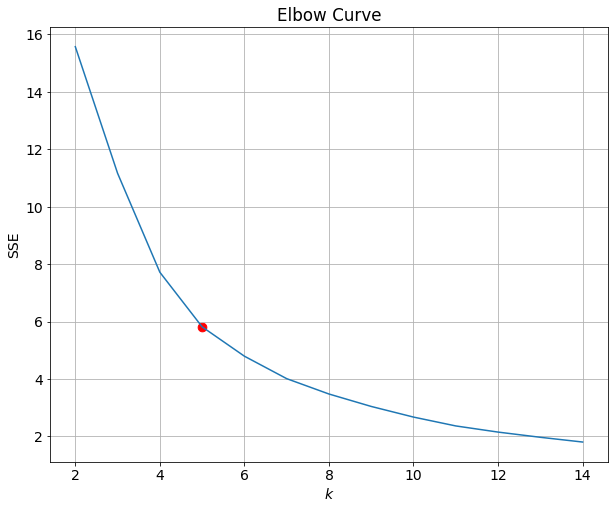
\includegraphics[width=0.7\textwidth]{figures/elbow_curve}
\caption{The eblow curve for the studied example.}
\label{fig:elbow_curve}
\end{figure}

\begin{ipython} 
kmeans = KMeans(n_clusters=5).fit(X)
centroids = kmeans.cluster_centers_
\end{ipython}

\begin{figure}
\centering
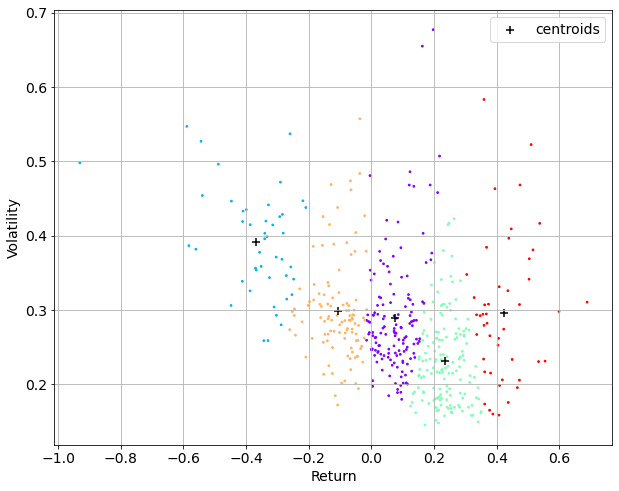
\includegraphics[width=0.7\textwidth]{figures/k_means_5}
\caption{The clustering results with the parameter $k$ equal to 5, black crosses represent cluster centroids. Note the outlier in the top right part of the plot.}
\label{fig:K_means_5}
\end{figure}
 
Fig.~\ref{fig:elbow_curve} shows also the presence of outliers as only one point is on the upper right side of the graph. This outlier form its own cluster. In order to have a better categorization of the stocks within the SP500 index, we would remove those stocks and fit the model another time.
This is done by finding the stock with the highest standard deviation value and dropping the corresponding columnn.
 
\begin{ipython}
stdOrder = ret_var.sort_values('Standard Deviation', ascending=False)
first_symbol = stdOrder.index[0]
ret_var.drop(first_symbol, inplace=True)
\end{ipython}
Then we can fit the dataset again, Fig.~\ref{fig:k_means_noout} reports the result.

\begin{ipython}
X = ret_var.values
kmeans = KMeans(n_clusters=5).fit(X)
centroids = kmeans.cluster_centers_
\end{ipython}
 
\begin{figure}
\centering
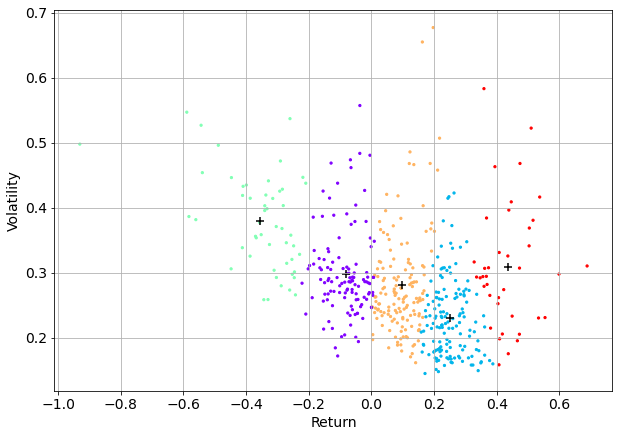
\includegraphics[width=0.7\textwidth]{figures/k_means_noout}
\caption{The clustering results after the outliers removal. The black crosses show each cluster centroid.}
\label{fig:k_means_noout}
\end{figure}
  
Finally we will assign to each stock its label (1, 2, 3, 4,and 5) and make a \texttt{DataFrame} with this information. Having the information of cluster number for each stock, we can create a diversified portfolio in the long term, between stocks from different clusters.

\begin{ipython} 
stocks = pd.DataFrame(ret_var.index)
cluster_labels = pd.DataFrame(kmeans.labels_)
stockClusters = pd.concat([stocks, cluster_labels], axis=1)
stockClusters.columns = ['Symbol', 'Cluster']
\end{ipython}
 
As an example the following are the stocks belonging to cluster number 0.

\begin{ipython} 
print (stockClusters.loc[stockClusters['Cluster']==0, 'Symbol'])
\end{ipython}
\begin{ioutput}
6      ADBE
7       AMD
11        A
14      ALK
20      ALL
       ... 
465    VRTX
466     VFC
483     WDC
493     XYL
496     ZBH
Name: Symbol, Length: 145, dtype: object
\end{ioutput}

\subsection{Natural Language Processing}

K-means algorithm can also be used in Natural Language Processing (NLP)~\cite{bib:nlp} which is a subfield of artificial intelligence concerned with the interactions between computers and human language, in particular copes with the analysis of large amounts of natural language data.

In there words (or sentences) are transformed into a set of numbers which then can be clustered together with k-means methods for a sentiment analysis of the text.
 
\begin{thebibliography}{9}
\bibitem{bib:smot}Nitesh Chawla, et al., \emph{SMOTE: Synthetic Minority Over-sampling Technique.}, 2012
\bibitem{bib:sensitivity}\href{https://en.wikipedia.org/wiki/Sensitivity_and_specificity}{\emph{Sensitivity and specificity}}, [Online]
\bibitem{bib:k-means}\href{https://en.wikipedia.org/wiki/K-means_clustering}{\emph{k-means clustering}}, [Online]
\bibitem{bib:elbow_curve}\href{https://en.wikipedia.org/wiki/Elbow_method_(clustering)}{\emph{Elbow Method}}, [Online]
\bibitem{bib:nlp}\href{https://www.ibm.com/cloud/learn/natural-language-processing}{\emph{Natural Language Processing}}, [Online]
\end{thebibliography}